\chapter{System concept and relevant aspects at a glance}

\begin{figure*}[!t]
	\centering
	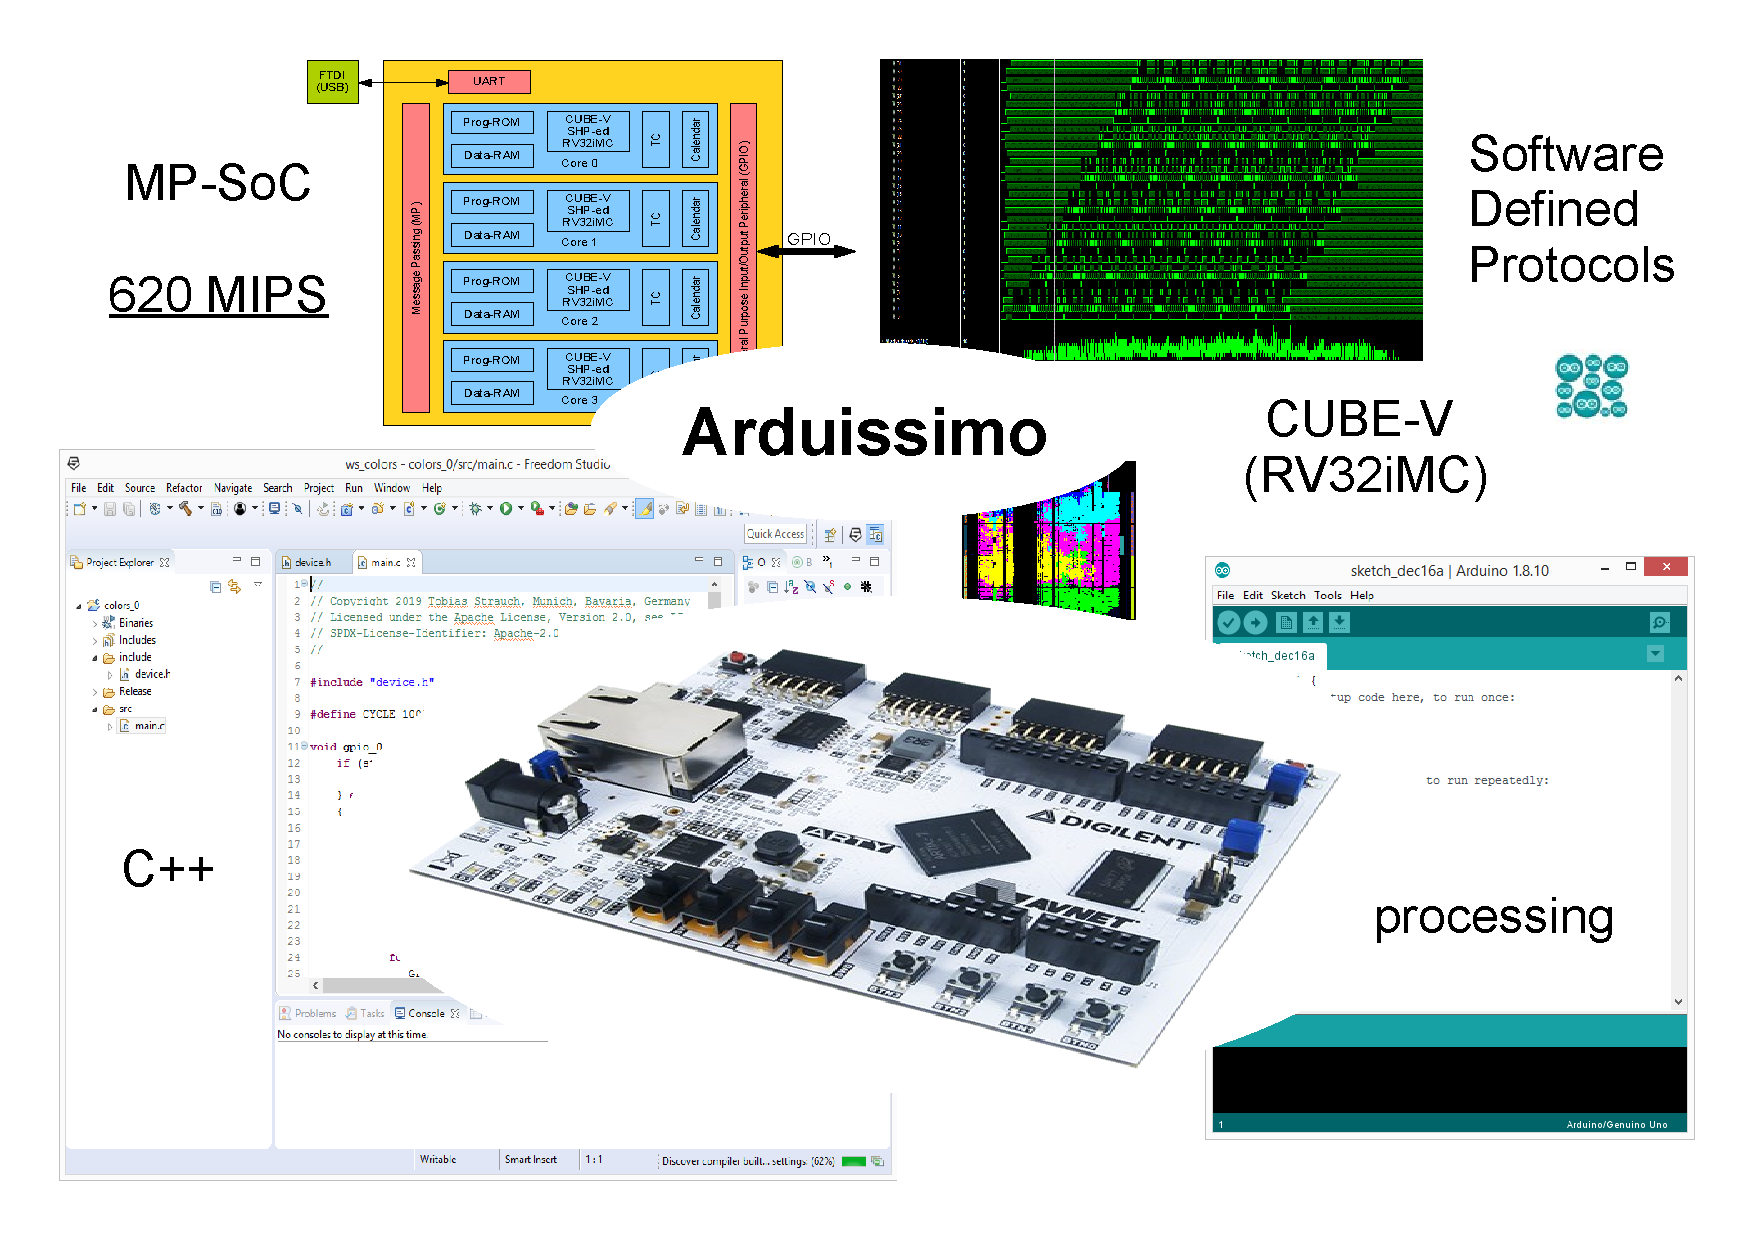
\includegraphics[width=6in]{figs/bigPicture}
	\caption{The big picture.}
	\label{overview}
\end{figure*}

For those of you, who don't want to read the complete doc, so basically all of you, here are the key aspects of this project:

As already mentioned, the projects is created to demonstrate the benefits of system hyper pipelining (SHP). We have 4 “CUBE-V” cores which run RISC-V 32-bit compatible code. Each one has 3 pipeline stages (“P3”). The complete design runs at 180MHz.  This clock generates what we call a micro-cycle. We applied C-Slow-Retiming \url{http://www.cloudx.cc/csr.html} generating 4 copies of each CUBE-V core (“C4”). It therefore takes 4 micro-cycles to finish one functional cycle, or in other words one macro-cycle is equal to 4 micro-cycles. We then apply the final SHP-step, using a memory depth of 16 lines (“D16”) to be able run up to 16 threads at the same time on each core in a time sliced fashion. 

The number of active threads can be changed dynamically. When less or equal 4 threads are executed, then each thread runs at a macro-cycle speed of (180MHz / 4 =) 45 MHz. When more than 4 threads are active, let's say n, then each thread runs at a macro-cycle speed of 180MHz / n. So for n = 10, to make is easy for you, each thread runs at 18 MHz.

A thread can be started by another thread or by a peripheral. There are no interrupts in the sense that a running program is interrupted, instead a new thread is started without affecting active threads (except timing-wise when n \textgreater= 4, as mentioned before). Only a thread can kill itself.

You can program at which program address a thread is started. So a thread can say, my dear thread controller, please start a new thread at 0xC0DE. You can also program any peripheral to start a new thread at a start address of your choice. You can also provide the new thread some extra information (like a task identification number for instance), which is automatically written into the link register a0 of the RISC-V register file. For example, in the a0 register the GPIO pin number is written, when an edge is detected at that given pin number.

Each core has a calendar, which can be seen as a complex timer. So you can program a list of future events into the calendar, which automatically sorts these events in a timely order and starts a thread at a programmable address, once the time for that event has come.

The CUBE-V core is based on the RV32IMC ISA, but the FENCE, ECALL and EBREAK instructions are not implemented. Also no control and system registers (CSR) are implemented.

The CUBE-V core achieves 0,86 IPC (instructions per cycle, here macro-cycle) based on the CHStone testcases. This relative high number comes from the fact, that register values are not only written into the register file (RF), but also applies already at the output of the RF when “needed” in the next cycle, so a RF-writethrough is implemented if you want. With an IPC of 0,86 one core reaches 155 MIPS at 180 MHz. Therefore 620 MIPS can be reached on the quad core setting that fits on the selected FPGA board.

The project is served on a bed of Windows project files with some Verilog strings attached.
